%
% LaTeX template for prepartion of submissions to PLDI'16
%
% Requires temporary version of sigplanconf style file provided on
% PLDI'16 web site.
% 
\documentclass[pldi]{sigplanconf-pldi16}
% \documentclass[pldi-cameraready]{sigplanconf-pldi16}

%
% the following standard packages may be helpful, but are not required
%
\usepackage{SIunits}            % typset units correctly
\usepackage{courier}            % standard fixed width font
\usepackage[scaled]{helvet} % see www.ctan.org/get/macros/latex/required/psnfss/psnfss2e.pdf
\usepackage{url}                  % format URLs
\usepackage{listings}          % format code
\usepackage{enumitem}      % adjust spacing in enums
\usepackage[colorlinks=true,allcolors=blue,breaklinks,draft=false]{hyperref}   % hyperlinks, including DOIs and URLs in bibliography
% known bug: http://tex.stackexchange.com/questions/1522/pdfendlink-ended-up-in-different-nesting-level-than-pdfstartlink
\newcommand{\doi}[1]{doi:~\href{http://dx.doi.org/#1}{\Hurl{#1}}}   % print a hyperlinked DOI


\usepackage[usenames,dvipsnames]{color}
\newcommand{\ruzica}[1]{\textcolor{Magenta}{\textsf{RP}: #1}}
\newcommand{\markk}[1]{\textcolor{Blue}{\textsf{MS}: #1}}
\newcommand{\alex}[1]{\textcolor{Orange}{\textsf{AR}: #1}}
\newcommand{\marvin}[1]{\textcolor{Green}{\textsf{MQ}: #1}}


\usepackage{comment}

\usepackage{graphicx}

\lstset{
  basicstyle=\footnotesize,
  breaklines=true,
  framextopmargin=50pt,
  frame=bottomline,
  language=haskell}
%\usepackage{minted}
%\usepackage{tcolorbox}
%\usepackage{etoolbox}
%\BeforeBeginEnvironment{minted}{\begin{tcolorbox}}%
%\AfterEndEnvironment{minted}{\end{tcolorbox}}%

\begin{document}

\title{Instructions for Submission to PLDI'16}

%
% any author declaration will be ignored  when using 'pldi' option (for double blind review)
%

\authorinfo{Person 1 \and Person 2}
{\makebox{A Department} \\
\makebox{A University}  \\
\makebox{A Place, AS 12345}}
{\{person1,person2\}@cs.auniv.edu}



\maketitle

\begin{abstract}
  We present programming by example that can utilize user defined higher order functions through a dismantling procedure.
  We use refinement types to prune the search space of higher order functions.
  Since our refinement types can be under approximating, we can extend liquid Haskell to support arbitrary syntax extensions and maintain soundness.
  for component/first order functions, we use type directed synthesis.
  We might use results from paramatricity to synth first order fxns, but probably not.
\end{abstract}


\section{Introduction} \label{intro}
(1) We use refinement type based inductive generalization (inductively deriving properties from examples).

(2) from the higher order examples we use deductive reasoning to automate refinement type inference on higher order function.

(3) We combine these two with abductive reasoning to create a ranking and perform a best-first enumerative search based on type closeness and code locality. 



\section{Motivating Examples} \label{examples}
As an introduction to \ourTool/, imagine that a user wants to synthesis the simple \codeinline{stutter} function that will duplicate each element of a list.
The user will provide an example, and \ourTool/ will synthesis a program \codeinline{concatMap (replicate 2)} that fit that example.

\begin{lstlisting}
exs :: [[Int] :-> [Int]]
exs = [[1, 2, 3] :-> [1, 1, 2, 2, 3, 3]]
\end{lstlisting}

We might also imagine that the user was able to complete a piece of this program by writing a function \codeinline{dupl} to duplicate an element. Now \ourTool/ will provide the solution \codeinline{concatMap dupl}, as well as the solution above.

\begin{lstlisting}
dupl :: a -> [a]
dupl x = [x,x]
\end{lstlisting}

Because \ourTool/ only searches for natural and idiomatic programs that use higher order functions, very few examples are needed. In this case the user wants a function that will take numbers from a list as long as the numbers are odd. Only a single example is needed for \ourTool/ to unambiguously find the function \codeinline{takeWhile odd}. Another valid function might be \codeinline{head} to take the first element. Searching for first order functions is an active research direction, but in this work we instead focus only on higher order functions. A discussion of integrating our tool with first order searching techniques in provided in Section \ref{evaluation}.

\begin{lstlisting}
exs :: [[Int] :-> [Int]]
exs = [[1, 2, 3] :-> [1]]
\end{lstlisting}

Working on user defined datatypes is also a commonplace task \ourTool/ supports. In the next example the user has provided a binary tree data structure and a function to map over it. For the sack of brevity, we show the synthesis the exceedingly simple program \codeinline{mapBTree not}.

\begin{lstlisting}
data BTree a = Nil |
               Branch (BTree a) a (BTree a)

mapBTree :: (a -> a) -> BTree a -> BTree 
mapBTree f Nil = Nil
mapBTree f (Branch b1 v b2) = 
  Branch (mapBTree f b1) (f v) (mapBTree f b2)

exs :: [BTree Bool :-> BTree Bool]
exs = [Branch Nil True Nil :->
       Branch Nil False Nil]
\end{lstlisting}

It may seem that if a user can write a higher order functions over custom data structures, they would not have a need to synthesize such functions.
However, imagine the incredibly common case of a user importing libraries.
Haskell's module system and large repository of libraries like Hackage and Stackage are an indispensable part of the language\cite{hackage,stackage}.
Often, a user is importing a library that is large, unfamiliar, and/or poorly documented.
Using \ourTool/, the user no longer needs an intimate knowledge of the library to makes use of the functions and datatypes, and can instead synthesize functions from examples.

As an example, we show code to transpose a music value from the Euterpea DSL for music\cite{Euterpea}.
Among other things, Euterpea defines a tree-like datatype called \codeinline{Music} and various functions for manipulating these types.
The user only needs to express the basic datatype as examples, and \ourTool/ can synthesize the \codeinline{solution} program.
The solution utilizes the functions from Euterpea; \codeinline{mMap} for mapping over music values, and \codeinline{(trans::Int->Music Pitch->Music Pitch)} to transpose a Music Pitch by a value.
Because we have synthesized a natural looking program, the user does not need to understand details of the library's function and data structures to be able to immediately gain an intuition about how the solution program works.

\begin{lstlisting}
import Euterpea

exs :: [Music Pitch :-> Music Pitch]
exs = [
  (Prim (Note qn (C,4)):+:Prim (Note qn (D,4)) :->
  (Prim (Note qn (D,4)):+:Prim (Note qn (E,4)) ]
        
solution = mMap (trans 2)
\end{lstlisting}

\markk{should we list the solution program that lambda squared would give? It would be long and full of cases and folds and maps}

\section{Problem Formulation}
In this section we formally define the space of functions we are interested in synthesizing. Using this definition we will show in section \ref{sound}, that although our algorithm is not complete in general (by the inherent nature of examples), it is complete for the subset of the language we define here.

We are interested in synthesizing higher order functions that manipulate data structures. We support the classic functions like \texttt{map, filter, foldl}, but also user defined higher order functions from user code, or imported modules. 

\begin{lstlisting}
solutionProgram ::
       (* -> types)  -- Component Function
    ->  types        -- Initial Values
    ->  *          -- Input
    ->  *          -- Output

types = * | * -> types

-- * matches on Type Variables and Constructors
\end{lstlisting}

We do not explicitly address synthesizing first order functions to fit the examples. We do employ a method to synthesize first order functions to act as the component functions for higher-order functions. Existing work has shown promising advances in synthesizing top level, first order functions\cite{potential, reviewers}. While it is out of the scope of this paper to go into details, we briefly discuss integration of dedicated first order synthesis procedures into our tool in section \ref{conclusions}.


\subsection{Example Syntax}
The user must give examples as a pair of values. We use the \texttt{:->} operator for clarity to differentiate between tuples and examples.
We require all higher order functions be be of a unified signature \texttt{$\_ \to * \to *$}, where the penultimate kind of the signature is the input and the final kind is the the output. \markk{Put in a note about data kinds here.} 

Functionally, this means we require that the user partially uncurry any higher order function they are interested in using during synthesis. This is a simple procedure, but requires user knowledge of which parameters to the function will be given by the examples. As an example consider 

\begin{lstlisting}
zipWith' :: (a -> b -> c) -> ([a],[b]) -> [c]
zipWith' f (xs,ys) = zipWith f xs ys
\end{lstlisting}

Any types that are between the input and first order function will be assumed to be initial values for the recursions. For example, \texttt{foldl (+)} needs an initial value of 0 to become the sum function.

%The liquidHaskell predicate applied to this signature will be of the effect of \texttt{len([a],[b]) = len([c])}.

\section{Implementation}


\begin{figure}[t]
  \centering
  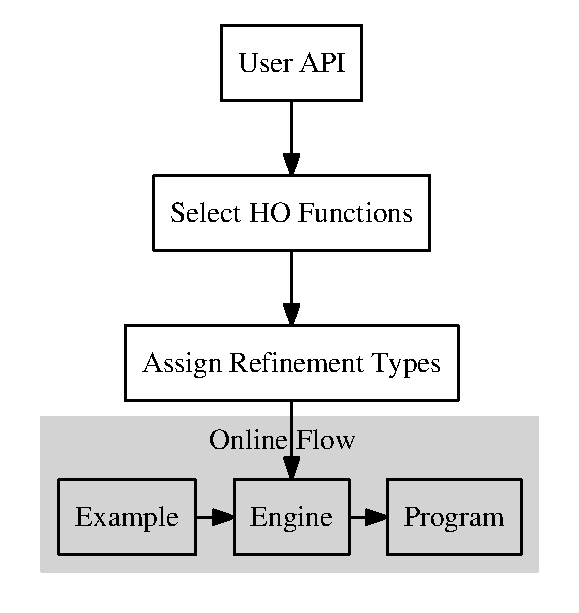
\includegraphics[width=0.4\textwidth]{algo}
  \caption{High-level structure of the algorithm.}
  \label{fig:high_level_overview}
\end{figure}

Figure~\ref{fig:high_level_overview} gives a high-level description of ways in which the components of our algorithm interact. Broadly speaking, there are two main stages in the algorithm. The offline phase gathers the higher order declarations visible in the APIs and user-provided code, and assigns refinement types to them to build a custom synthesis \textit{engine}. This engine is then used during the online phase of the algorithm to search for functions that fit a set of supplied examples.

During the offline phase, the algorithm first scans the user-provided code, the libraries it imports, and the standard library to gather all of the functions and global values visible to the program. Then, it selects the higher-order functions from the set of all functions and values, and uses Liquid Haskell \cite{liquidhaskell} to assign refinement types to each one. Finally, each higher-order function is assigned a weight based on locality. User-defined functions are given the highest priority, while direct imports are given less, and the standard libraries are given the least. Together with the first-order functions and values, these triples of higher-order functions with their refinement types and weights are collected to produce a synthesis engine.

Once this stage is complete, the user can make online queries to the synthesis engine, which will search the space of constructable functions for those that fit the input examples. First, the engine computes a refinement type that fits the examples. This type is matched against the refinement types of the known higher-order functions, and the weights of each known function are adjusted based on how close the types match, if at all.

Once the candidate higher order functions have been chosen, the synthesis engine performs a best-first search for a program that fits all of the input and output examples by composing the candidates with first-order functions. For example, the higher-order function \texttt{map} might be supplied the \texttt{length} function if the example inputs are lists of lists of integers and the output examples are all lists of integers. The programs that are examined during the search are evaluated against the example set and are reported to the user as they match. Because the weights favor local declarations, the highest-ranked programs are likely to be the most idiomatic.

\markk{explain each of these lines in the rest of the paper, citing line numbers. once all of the lines are covered here we are done}

\begin{lstlisting}[caption=A pseudocode representation of the build and synthesis stages of the synthesis algorithm. We will explain each line of this in the proceeding sections., label=listing:Algo]
main = do
  eng <- build
  ex  <- getExamples
  synth eng ex
  
build = do
  allTypes   <- collectTypesAndWeights
  allHOTypes <- filter isHigherOrder allTypes
  allRTypes  <- assignRTypes allHOTypes
  return (allTypes,allRTypes)
  
synth eng ex = do
  -- assign examples a refinement type too
  exType   <- getExampleType ex
  exRType  <- if   sameInOut exType
             then assignRTypes exType
             else noRType
  -- make candidate functions and programs
  hoFxns <- rankByTypeMatch exRType eng
  progs  <- makeFxns exType hoFxns
  -- test the ranked list of possible programs
  validProgs <- filter (testOn ex) progs
\end{lstlisting}


\subsection{Offline: Synthesis Engine Construction}
\subsubsection{Refinement Type Generation}

%>  filter ishigherOrder tys
We first collect all of the type signatures from our sources (user code, imports, and standard library). We filter through these to select only the higher order functions. Because in Haskell the function type constructor (->) is right binding, any higher order functions must have parenthesis in the type signature, which provides a convenient filtering predicate.

%> let uHOTyps = f 3000 typSigs
%> let iHOTyps = f 2000 importSigs
%> let pHOTyps = f 1000 preludeTypSigs
In order to rank the higher-order functions, we assign weights based on their source location. User-defined functions are given the highest priority, while direct imports are given less, and the standard libraries are given the least. These rankings will contribute to the final ranking of candidate functions in the synthesis stage when we match the component function signatures on the examples.

%> hoRTyps <- mapM (addRType fc) (map fst allHOTyps)
%> HigherOrderFxn -> (injectRFxnType fxn .fst)
We automatically generate refinement types for our higher order functions that will be used to prune the search space in synthesis.
In the case that the input and output types of the higher order functions are the same (up to the top level type constructor), we generate a LiquidHaskell predicate that relates the size of those types.
the size relation that applies to the higher order functions must also apply to the examples in order to consider that function as a candidate.   

In the case that the input and output type are different, we note that the size measures between two different type constructors are not guaranteed to have any significance.
A relation on these values may be useful on occasion, but in practice is often only a confounding factor.
Since LiquidHaskell is the largest cost to our system, removing refinement type inference in these ambiguous cases provides a large performance gain.
In processing the Haskell standard library, base:Prelude, we remove \markk{FILL ME IN} cases of refinement type checking.
Hypothesis generation about these higher order functions is then deferred to the synthesis stage and where we use a subtype ranking system to good effect.

In order to derive these refinement types, we require all higher order functions be be of a unified signature \texttt{$\_ \to * \to *$}, where the penultimate kind of the signature is the input and the final kind is the the output. \markk{Put in a note about data kinds here.} Functionally, this means we require that the user partially uncurry any higher order function they are interested in using during synthesis.

This is a simple procedure, but requires user knowledge of which parameters to the function will be given by the examples. 
As an example consider 

\begin{lstlisting}
zipWith' :: (a -> b -> c) -> ([a],[b]) -> [c]
zipWith' f (xs,ys) = zipWith f xs ys
\end{lstlisting}
%The liquidHaskell predicate applied to this signature will be of the effect of \texttt{len([a],[b]) = len([c])}.


%> map rTypeTemplate ["=","<=",">="]
When the input and output types are the same, or use the same top level type constructor, we generate hypotheses as liquidHaskell predicates.
Our predicates specify size constraints on input and output of $\leq,\geq,=$.
For every predicate provided, we are able to more accurately prune the search space of higher-order functions, but we must test every higher-order function in scope on these predicates. 
Therefore, it is best to only select as many refinement types as is needed.
Although this offline stage only needs to be run once given a set of code and imports, liquidHaskell type checking is still fairly expensive.



\subsubsection{User defined data types}
%We focus only higher order functions that manipulate data structures
In order to support user defined data structures, we only require that a user implements some kind of measure\cite{realWorldLiquid} over their data structure.
This size function will help the system determine size constraints on the examples, so that we can pick higher order functions that might actually work.
In fact, a size function could just be a constant function, which means the system will test every higher-order function that fits the types. 
\markk{Maybe this should even be a builtin default? If liquid haskell says no def for len, just set the type to true - thats an easy hack}

As an example, take the code from section \ref{examples} for synthesizing a music function.
the user would have needed to provide a measure function for Music a.
This measure will allow liquidHaskell to draw conclusions about the size of examples of type [Music a :$\to$ Music a], as well as conclusions about higher order functions over the Music data structure.

\begin{lstlisting}
import Euterpea

{-@ measure len @-}
len :: Music a -> Int
len m =
  case m of
    Prim _  -> 1
    m1 :+: m2 -> len m1 + len m2
    m1 :=: m2 -> len m1 + len m2
    Modify c m -> len m
\end{lstlisting}





\subsection{Online: Fitting Functions to Examples}
Once the synthesis engine has been constructed, the system is ready to answer function fitting queries. When examples are provided, the synthesis engine finds a suitable refinement type for a hypothetical function that could fit that example. Then, this refinement type is matched via builtin type-checking against the higher order functions known to the engine.

Once the candidate functions are identified, a best-first search is initiated over combinations of the higher-order functions curried with each component function so that the combination type-checks. Each of these is executed against the set of inputs. Whenever a function produces the correct outputs for each input, it is said to fit, and is reported to the user. This search continues until the space is exhausted or it is manually interrupted.

As in section \ref{HORtypeInf}, we also consider two cases for examples. The first where the example input and output types match up to the top level type constructor, and the the case where the types do not match.

In the case that the types do match, we find the set of refinement types that the examples satisfy. Generating refinement type predicates about the size of the input and output, as in section \ref{HORTypes}, we run type inference on the input / output examples to \markk{ALEX, the following is wrong, what is a basic rtype anyway?} get a basic refinement type. Then, the input-output pairs are matched against a fixed set of predicates to enrich the refinement type. These predicates could impose constraints such as the input list being of equal, lesser, or greater size to the output list. \markk{end things being junk} For instance, the example set:
\begin{minted}{haskell}
exs = [[1,2,3,4] :-> [1,3],
       [2,4,6,8] :-> [],
       [5,7] :-> [5,7]]
\end{minted}
\noindent would have an inferred base type \markk{this isn't inferend right now, if we want to do that we would be using ghc, not LiqHask. check http://stackoverflow.com/questions/8963488/automatically-add-type-signatures-to-top-level-functions for a script to test} of \texttt{[Int] -> [Int]} and its final refinement type would be \texttt{xs:[Int] -> \{ ys:[Int] | len xs >= len ys \}}, since all of the examples suggest that the output list does not grow. The addition of these refinement type predicates dramatically reduces the search space in practice.

Once these higher order functions have been culled from the pool of candidates, we iterate through each in best-first order. For each higher-order function, we supply it with arguments until it is compatible with the type signature implied by the example set. By convention, we take the final argument of the function to be the input, which means that higher-order functions that take multiple inputs have to explicitly be uncurried. Value types are satisfied by selecting from a pool of default values, and function types are satisfied by searching for first-order functions that would make the resulting signatures match. If it is not possible to find values that fit, the search moves on to the next higher-order function.

\subsection{Dismantling procedures}

A \textit{dismantling procedure} prunes the first order function search space.
Subexample generation from that other paper\cite{isil} is one example of a (powerful) dismantling procedure. Subexample generation also gives the ability to recursively call the synthesis engine to generate programs with multiple applications of a high order function.
Because subexample generation is hard, and we dont know how to do it yet, we present a different idea.
Our dismantling procedure will deduce a specialized component signature given a higher order signature and the examples signature.

To choose the component function we use a sound, but not complete subtyping.
When two types have this relations, we will say type a \textit{generalizes} type b.
\markk{someone probably wrote something about this, just need to find out where and cite.}
If we have the higher order function map :: (a$\to$b) $\to$ [a] $\to$ [b] and the examples :: [Int] $\to$ [Int], then our component function f might have f::a$\to$b, or f::Int$\to$Int, or f::Int$\to$a, but certainly not f::[Bool]$\to$[Bool].

\begin{minted}[fontsize=\footnotesize]{haskell}
map :: (a -> b) -> [a] -> [a]
exs :: [Int] :-> [Int]

--component function must generalize
f :: Int -> Int

goodFxn1 :: Int  -> Int
goodFxn2 :: Int  -> a
goodFxn3 :: a    -> a
badFxn   :: Bool -> Bool
\end{minted}

\subsection{Handling folds}
We identify two separate classes of higher order functions - those that take a single first order function, and those that need initial values in addition to a function. The \texttt{map} function only takes a first order function, while \texttt{foldl :: $(a\to b\to a)\to a\to [b]\to a$} requires an initial value for \texttt{a}. While the process described so far handles the former, initial values must also be addressed.

To identify initial values in a type signature, we can use our previous assumption that all hihgher order function have been partially curried to the type \texttt{$\_\to *\to*$}. Adding the further assumption that only one first order function maybe be passed to the higher order function, we simply tag any non-function type in the hole as an initial value. 

Since examples must be given as a concrete type, we can always specialize a our candidate higher order function. If the initial type is an instance of Monoid, we can extract the unit value (mempty in the moiod typeclass) to use as our initial value. 

For lists, the unit element is []. However, there are two valid monoids for numbers, using either (+) or (*) as the operators and resulting in unit elements 0 and 1 respectively. We take both of these values as possibilities since the cost is small \markk{compared to all the refinement type stuff we are doing.}

Requiring our users to write monoid instances may be a nuisance. Additionally, users may have some domain knowledge that a particular value may be useful in their applications of folds. If this is the case, users may write specializations of these functions to be used in synthesis. Since our system automatically considers functions defined in the user code base, \markk{finish sentence}.

\begin{minted}[fontsize=\footnotesize]{haskell}
--to use 5 as an initial value for foldl
foldl :: (a -> b -> a) -> [b] -> a
foldl5 f i o = foldl f 5 i o
\end{minted}


\subsection{Soundness and Completeness}
\markk{for completness, can we show that we are complete within a specific domain? Also see \ref{extLiqHask} for more on completness.}

From the procedure outlined above, it is clear that no function will be returned by the algorithm that does not fit the examples given, since functions are validated before being reported. Still, it is possible for the synthesis procedure to return a function that does not capture the user's intent. Generally, this can be solved by supplying more examples to narrow the set of possible fitting functions.

However, depending on what the user is trying to synthesize, and which examples have been provided, it is possible for new examples to increase the search space. If, for example, a user gives only positive examples for a \texttt{filter}, the refinement type predicate discovery will assume that the lists do not change size, and will likely return \texttt{map id} as a result.

On the other hand, the set of functions that the algorithm can produce is fairly broad. It is able to search through the entire space of higher order functions that have been specialized with a first-order function, when considering the functions that are in scope. We will see in section~\ref{sec:evaluation} how broad this space actually is.


\section{Evaluation}
here is a big table that takes up a whole page

\subsection{Optimizations}

Since the standard library can be considered a relatively stable set of code, we can cache the refinement type inference to reduce the build time.
On my machine, it removes ~40 seconds from the build time.

\section{Related Work and Conclusions}
\subsection{Limitations}

Without subexample generation we cannot recursively apply our algorithm to create programs with multiple applications of higher order functions as in the   $\Lambda^2$ paper\cite{isil}. Since they provide hard coded subexample generation hypotheses for the higher order functions they use, this does not scale.

With the eventual goal of building a complete program synthesis engine, we will need to integrate the first order function synthesis. While this problem has been investigated in isolation, it is not clear how to efficiently determine if  a set of examples will require a higher order function or a first order function.

The user must provide a concrete type signature for the examples. This could be fixed by making use of Haskell's monomorphism restriction and inline the inferred concrete type signature.

In providing initial values for component functions, we are strictly reducing the number of kinds in a type signature.
We could expand types, which would create an infinite recursion, but allow us to find many more functions.

\begin{lstlisting}
--given the component function
f :: Int -> Int
f = (+1)
--expand the type
f' :: Int -> Int
f' = f . (+1)

\end{lstlisting}


\subsection{Optimizations}

\subsection{Related}
Subexample generation from that other paper\cite{isil} is one example of a (powerful) dismantling procedure.
Subexample generation also gives the ability to recursively call the synthesis engine to generate programs with multiple applications of a high order function.
Because subexample generation is hard, and we dont know how to do it yet, we present a different idea.
Our dismantling procedure will deduce a specialized component signature given a higher order signature and the examples signature.

\bibliographystyle{abbrvnat}
\bibliography{sample}

\end{document}
